\section{\Compound{} DMA attacks}\label{sec:linux_net}

\adam{I'd retitle this section: it is about kernel design flaws to enable getting Motive, Means, and Opportunity}

%So far, we have demonstrated a \simple attack by exploiting type (a) \subpage vulnerability of the FireWire driver. 
In this section we explore new attacks on the Linux network stack where \means and \oportunity are initially missing but are attainable via compound steps.
%\st{, leaving room to dangerous privilege escalations attacks}.
We focus on the Linux network stack which initially seems secure \cite{thunder}. 
But, by \tool and as we demonstrate in this section, the Linux network stack is actually responsible for \%60 of DMA vulnerabilities we have found. 
We first describe the vulnerable data structures shared by \emph{all} Linux network drivers. We then show how \oportunity is often achievable. Then, we discuss various methods to achieve \means and \motivation. 
In the interest of space, additional DMA attacks also appear in \ref{appx:additional_compound}.

\subsection{\shinfo}
\begin{figure}[t]
    \centering
    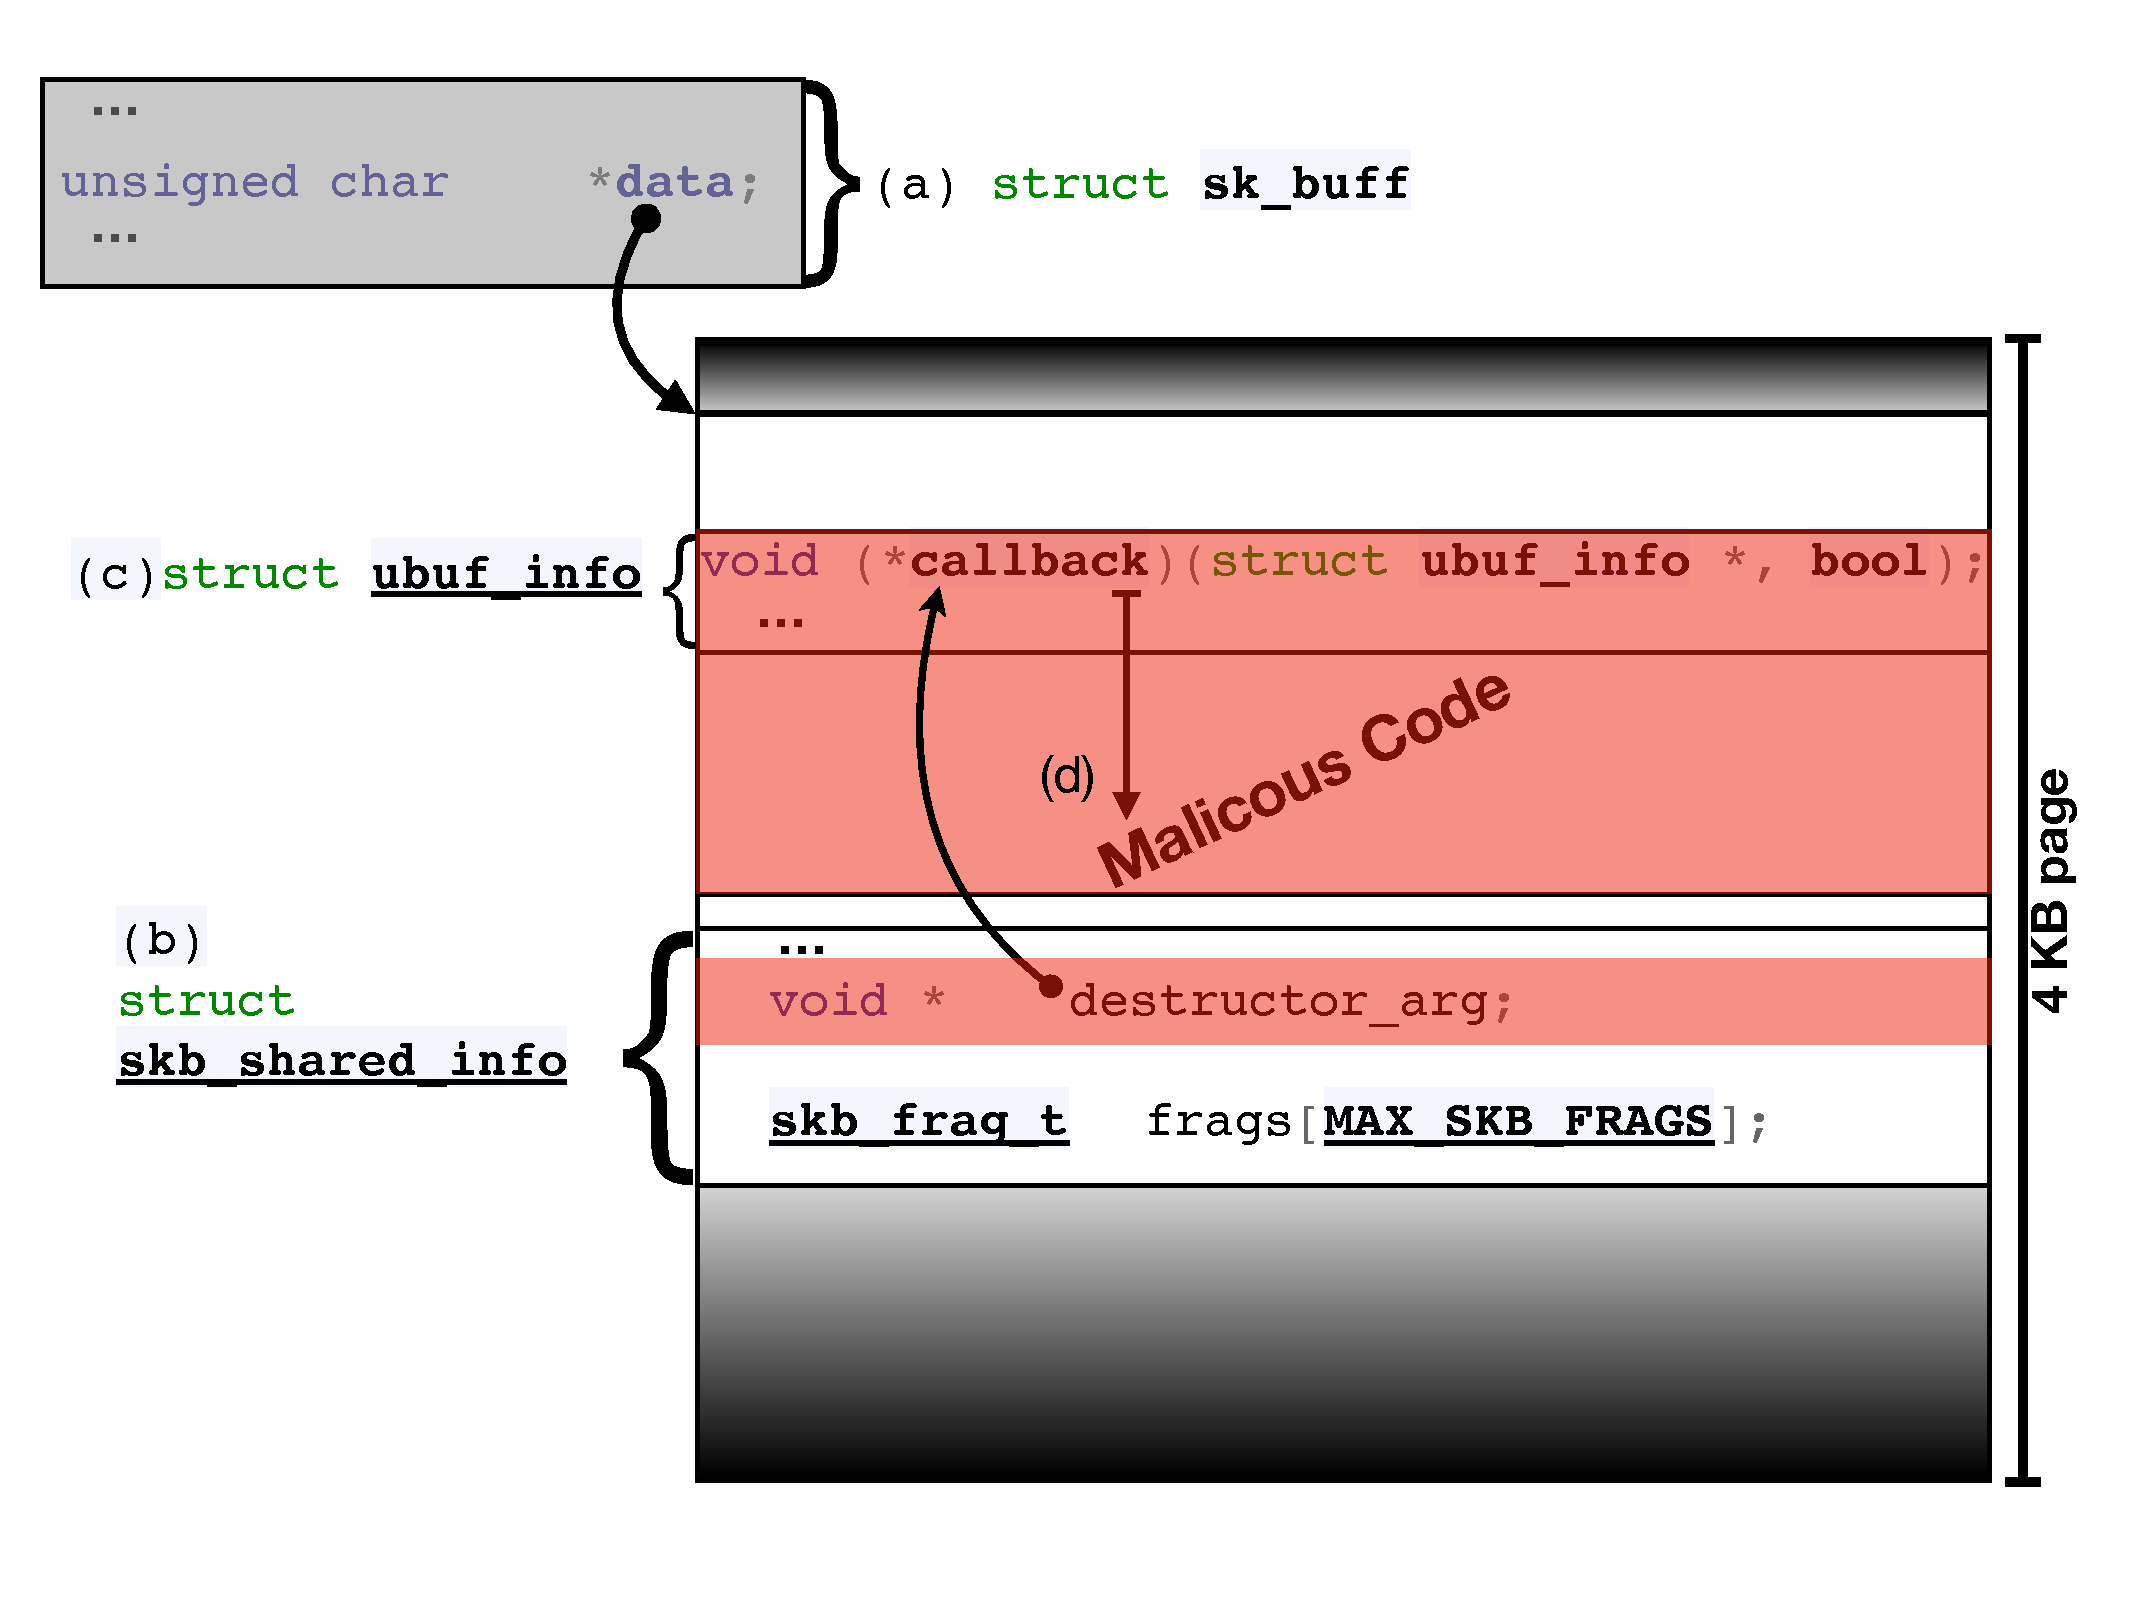
\includegraphics[width=\linewidth]{figs/ubuf.pdf}
    \caption{Using \shinfo{} to execute arbitrary code in kernel context.}
    \label{fig:sh_info}
\end{figure}

%\adam{lots of explanations here, whereas the structure was originally mentioned when talking about SCAT...}
Struct \skb{} is a data structure used by the Linux network stack to hold information representing a network packet. Struct \skb{} holds the metadata of a network packet (e.g., packet size, associated socket). One of these fields is a pointer to a data buffer. The data is allocated separately, and thus, does not share a page with its \skb{} (Fig. \ref{fig:sh_info}). 

This separation means that \skb{} is \emph{never} (intentionally) mapped to the device. Indeed, it is a common belief, pointed out in literature \cite{thunder}, that the Linux network stack is not susceptible to DMA attacks via the \texttt{data} pointer. In this work, we show that this belief is misplaced.

The Linux network stack supports packet cloning by merely copying \skb{} metadata. This includes the \texttt{data} pointer. That is, the resulting \skb{} and the original one share the data buffer \cite{drivers2005linux}. Note that the \texttt{data} buffer of the \skb{} is the \emph{linear} part of the payload but \skb{} also supports \emph{non-linear} buffers, i.e., buffers described by their \page{}, length and offset in the \texttt{frags} array of \shinfo{} (Fig. \ref{fig:sh_info}). 

To support these non-linear buffers, the \shinfo{} metadata structure is used.
Struct \shinfo{}, in contrast to \skb{}, is \emph{always} allocated as part of the data buffer. Therefore it is \emph{always} mapped to the device. \shinfo{} is unwittingly mapped with the permissions of the packet, i.e., WRITE for RX packets, READ for TX packets, and in some cases, such as XDP \cite{xdp} with BIDIRECTIONAL.

Consequentially, \shinfo{} is the potential \oportunity{} the malicious device has been looking for. The \subpage{} vulnerability created by \shinfo{}, represents a type (b) vulnerability (Fig. \ref{fig:colocation} (b)), as this is innate to Linux networking rather than a driver security bug. 

Fig. \ref{fig:sh_info} depicts how a malicious device can mount an attack using \shinfo{} in four steps:
\begin{enumerate}[label=(\alph*)]
    \item An RX \skb{} and its data buffer are allocated. The data buffer is mapped for the NIC with WRITE access (the WRITE access is to the whole 4~KB page). 
    \item \texttt{destructor\_arg} field in \shinfo{} is overwritten to point within the mapped page. Now, the \texttt{destructor\_arg} is pointing to struct \uarg{} which is created by the NIC.
    \item \uarg{} has a callback pointer that is now pointing to the malicious code residing on the same page. In the case of NX-bit, it is a poisoned ROP stack (Sec.~\ref{sec:nx-bit}).
    %\adam{how does this work? you overwrite a pointer to a callback function, not to the stack pointer.}
    \item when the \skb{} is released, the callback is invoked.
\end{enumerate}
To expand this scenario into a complete attack, the attacker must complete the MMO trifecta. That is, both \means{} (the attackers needs the actual \kva{} of the \mabaf{}) and \oportunity{} (the NIC must have a timely WRITE access to the page) are required. In the next subsection, we demonstrate how an attacker can leverage standard OS behavior to obtain both missing attributes.

\begin{figure}[t]
    \centering
    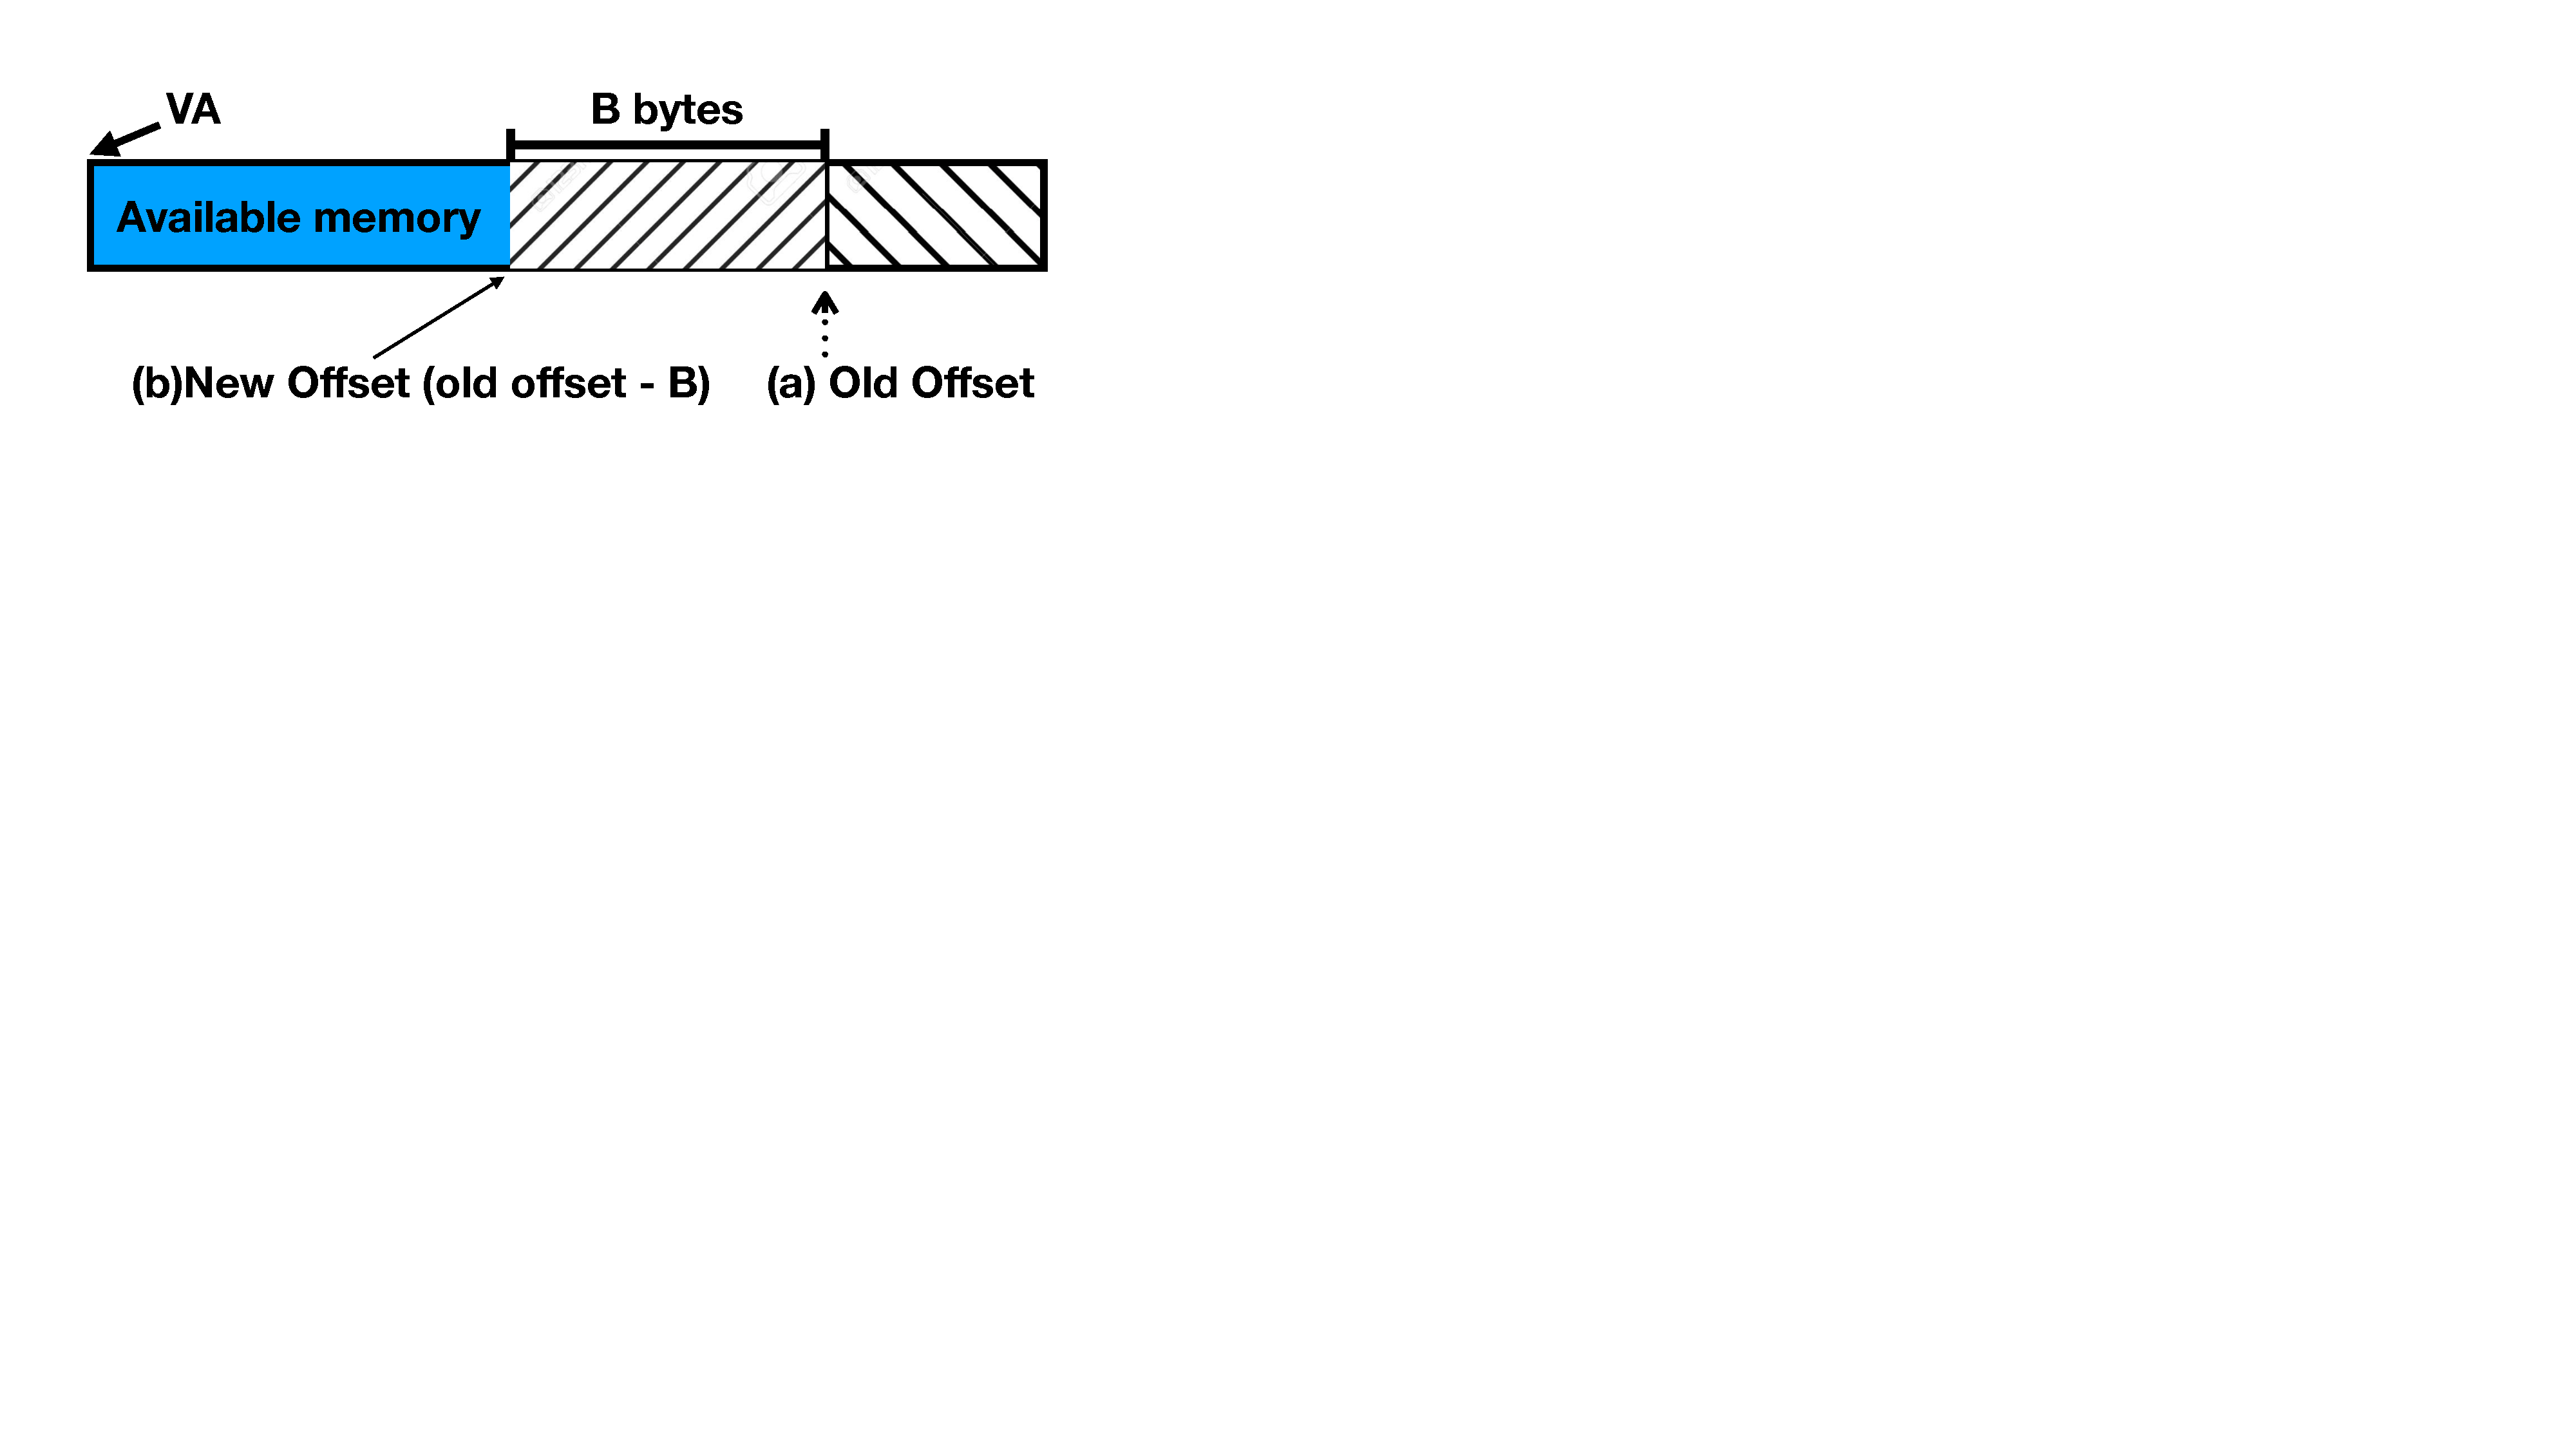
\includegraphics[width=0.8\linewidth,trim=0 6cm 0 6cm, clip]{figs/page_frag.pdf}
    \caption{Allocation of B bytes from page\_frag}
    \label{fig:page_frags}
\end{figure}

\subsection{Deferred Invalidation vulnerability}\label{sec:deferred}

To limit the overhead of multiple memory accesses when translating \iova{} using page tables, the IOMMU caches translations in an I/O translation lookaside buffer (IOTLB). 

The IOTLB is analogous to the MMU TLB. IOMMU does not maintain consistency between the IOTLB and the IOMMU page tables. As a result, the OS has to explicitly invalidate the IOTLB to maintain consistency when a translation entry is removed. Namely, to ensure that the IOTLB never holds stale entries, the OS must invalidate the IOTLB immediately after it removes memory mappings. 

Yet, this scheme, called the \emph{strict} mode in Linux, can degrade performance, as IOTLB invalidations can induce very high overhead \cite{MMT16,MSMT18,Peleg15}. In I/O intensive workloads, the number of required IOTLB invalidations can be extremely high, as IOMMU entries are unmapped following each I/O operation. Moreover, the overhead of each IOTLB invalidation can be as high as 2000 cycles \cite{ABYTS11}. This is considerably higher than a TLB invalidation, which takes roughly 100 cycles \cite{Han14}. 

To reduce this overhead, Linux defers TLB invalidations by default and instead performs periodic global TLB invalidations. While \emph{deferred} mode, improves I/O performance, it also breaks the stipulation, that after unmapping (e.g., \texttt{dma\_unmap\_page}), the physical page should no longer be accessible by the device. This \emph{deferred} time frame (Fig. \ref{fig:deferred}), may be as high as 10 milliseconds \cite{MSMT18}.

The repercussions of \emph{deferred} mode are that a malicious device can take advantage of this time window, where it has access to memory pages, effectively, unbeknownst to the CPU. This opens up two distinct attack options:

\begin{enumerate}
    \item A device can alter data structures that the CPU has modified \emph{after} unmapping (e.g., calling \texttt{dma\_unmap\_page}).
    \iova{} mappings, as a rule, are short-lived as they should be used only for the duration of I/O, usually for a few microseconds. The additional milliseconds provide the attacker with a wide time-window sufficient to conduct her attack.
    \item The page can be freed, and then immediately reused by the OS. In fact, this is a common scenario, as Linux reuses \emph{hot} pages (i.e., recently used pages), as they are likely, to already reside in the CPU caches \cite{hotcold}. In turn, this opens up the kernel to additional random access attacks.
\end{enumerate}

\begin{figure}[t]
    \centering
    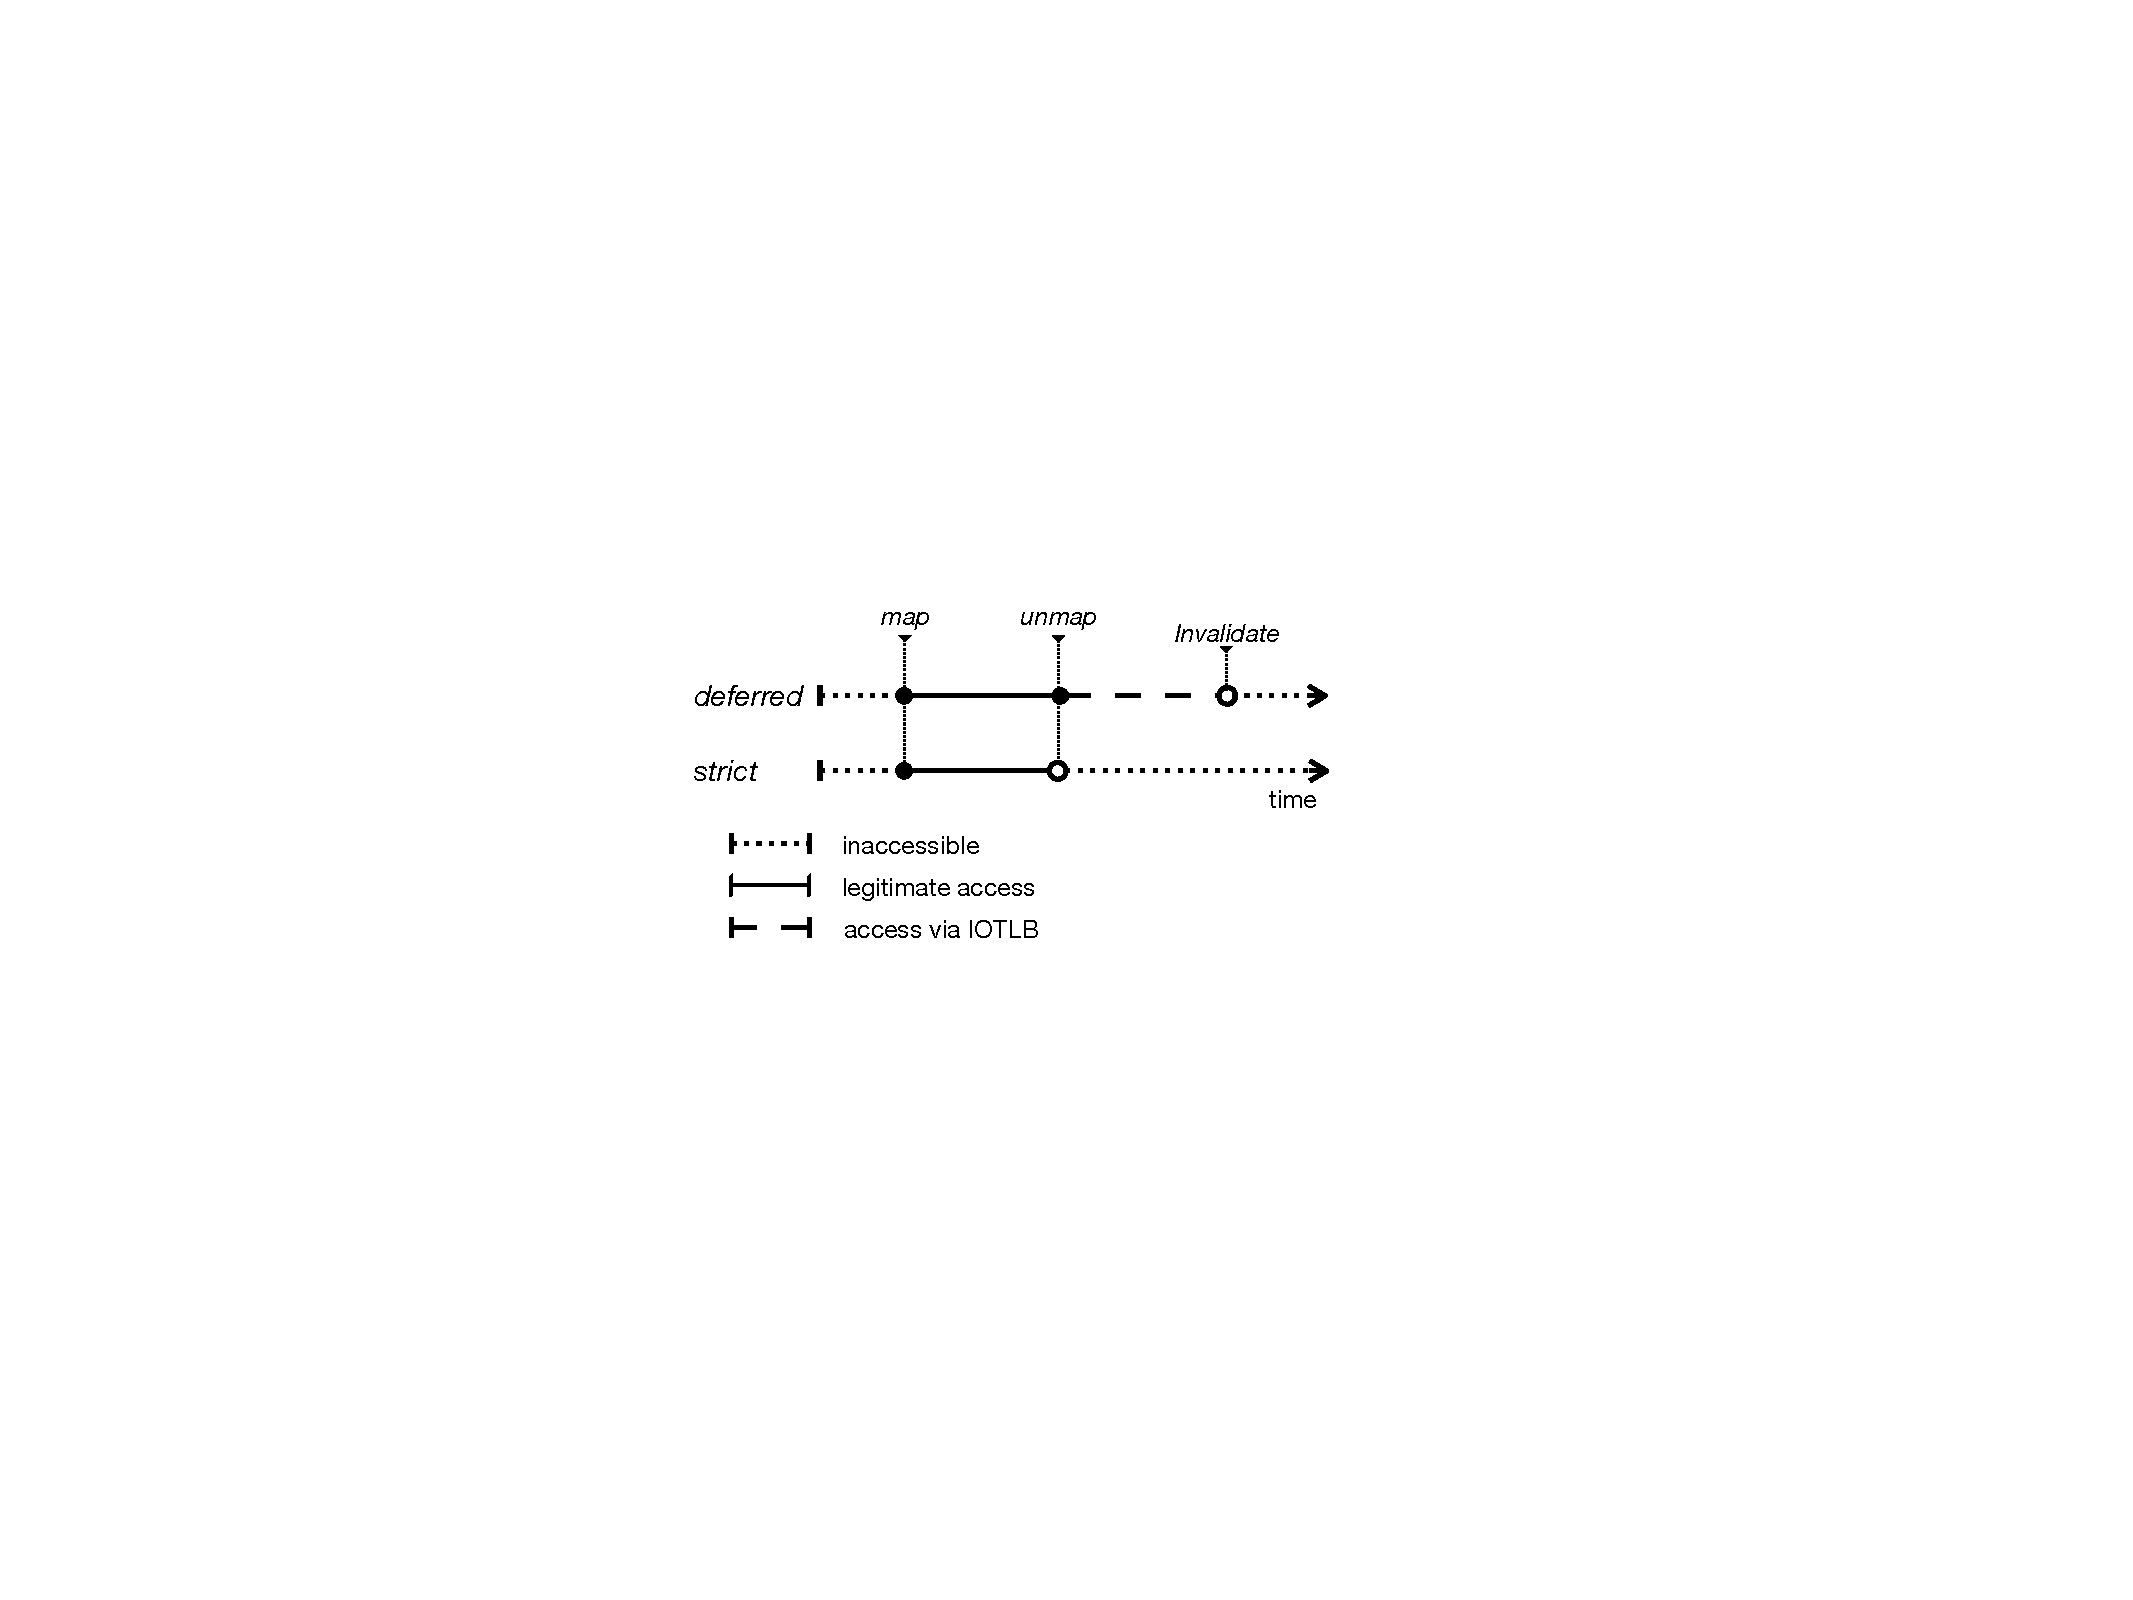
\includegraphics[width=0.9\columnwidth]{figs/strict.pdf}
    \caption{Strict vs. deferred IOTLB invalidation. In \emph{deferred} mode, there is a time window where the data is accessible to the device, but the mapping no longer appears in the page table.}
    \label{fig:deferred}
\end{figure}

\subsection{Hacking~\oportunity{}}\label{sec:shinfo}

\begin{figure}[t]
    \centering
    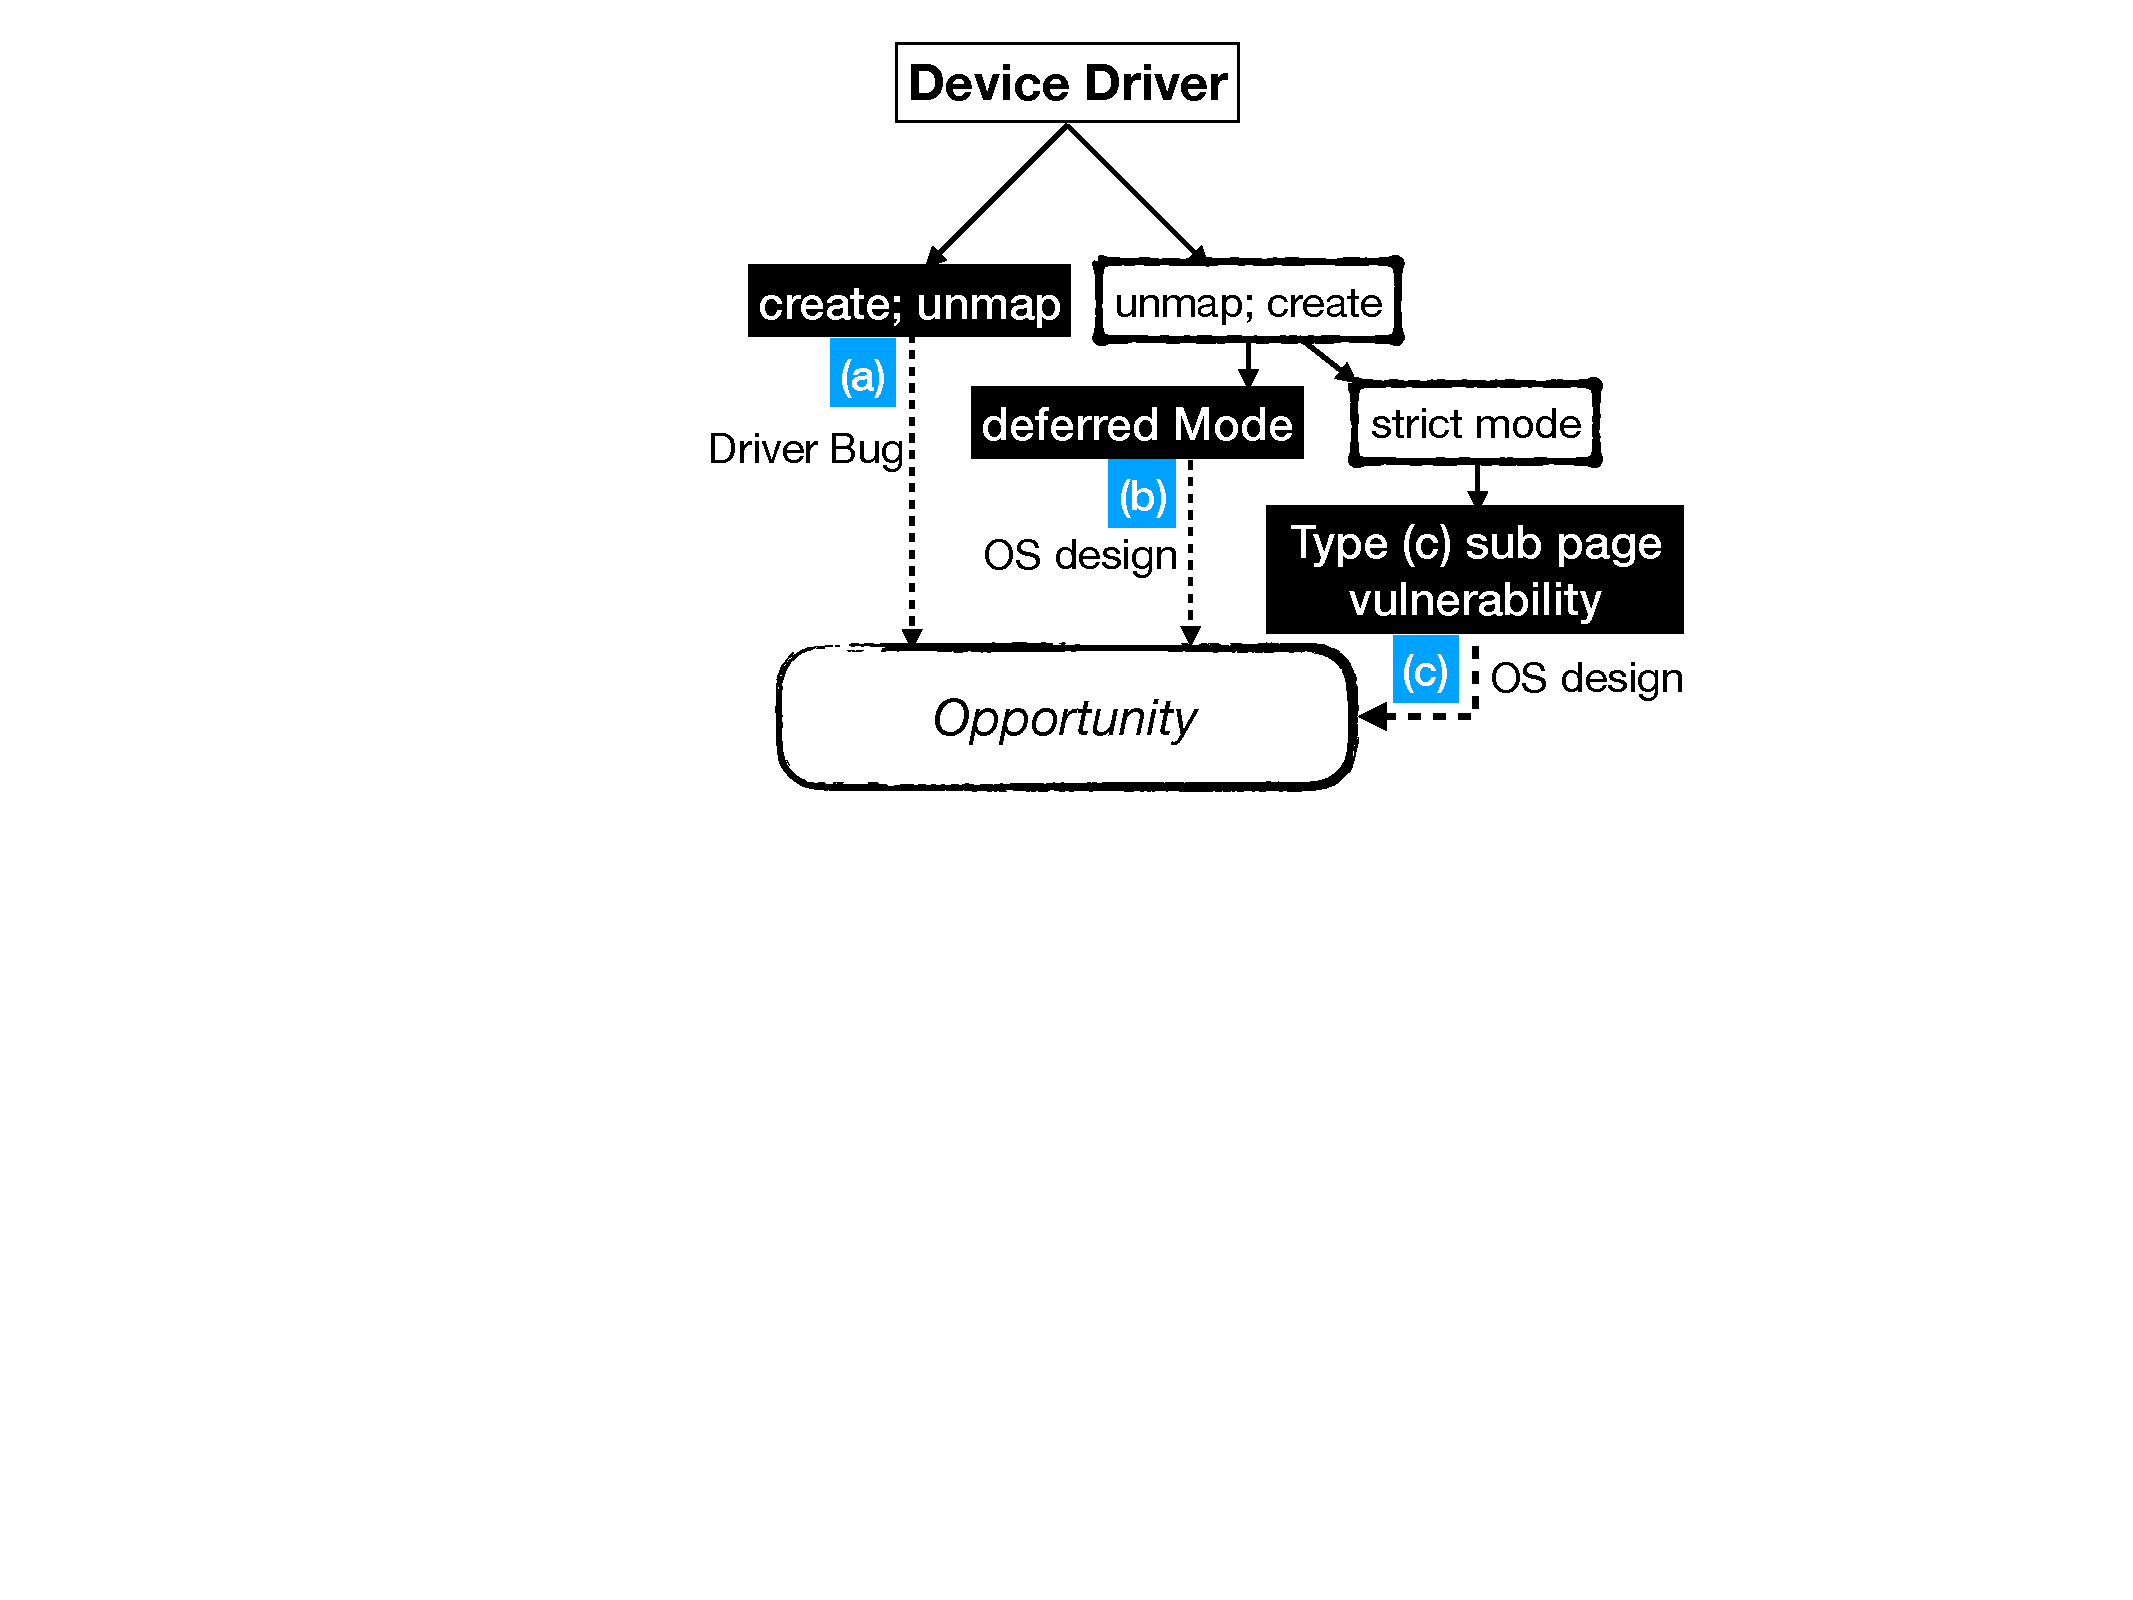
\includegraphics[width=0.8\linewidth]{figs/road_to_op.pdf}
    \caption{Different ways to obtain \oportunity.}
    \label{fig:road_to_op}
\end{figure}

\adam{IMPORTANT POINT: To me, it seemed that the tool sections were about gaining Opportunity.  Why do we now need another section on "Hacking" it? Do the tools not flag the skb-shared-info? If they do, and it's still not enough, how do we know Opportunity exists in the other cases they flag?  Perhaps, the exact goal of the tools and what they find should be described more precisely.}
We now detail the different ways in which a malicious device can obtain \oportunity{} (Fig. \ref{fig:road_to_op}).

\begin{enumerate}[label=(\roman*),wide, labelwidth=!, labelindent=0pt]

\item Presumably, a correct use of the DMA API should thwart the attack outlined in the previous section (Fig. \ref{fig:sh_info}). Namely, first unmapping the buffer and only then initializing the \shinfo{} should allow the CPU to undo any malicious changes the NIC may have perpetrated. 
As it turns out, prevalent device drivers (e.g., Intel 40GbE driver, i40e) first create an \skb{} and only then unmap the buffer. This order of execution allows the \emph{device} to undo legitimate changes to \shinfo{} by the CPU. 

\item Nevertheless, even when the order is correct, i.e., the unmapping of the buffer occurs before the creation of the \skb{}, still \shinfo{} is not safe from later modifications. As the default IOMMU mode in Linux is \emph{deferred} protection (Sec. \ref{sec:deferred}), the unmap order is made irrelevant. That is, even though the unmap function is invoked in the correct order, the device can still corrupt \shinfo{} due to the IOTLB.  \adam{instead of a backreference, S3.3 should be put here to describe the vuln}

\item In response, a security-conscious admin may change the default setting to \emph{strict} mode, where the IOTLB is flushed on every unmap. However, this both severely degrades networking performance \cite{MMT16,MSMT18}, and does not alleviate the security threats on the system. Presumably, with \emph{strict} mode enabled, the \iova{} the NIC used to access that \shinfo{} is no longer valid, which initially sounds promising. The problem is that the device, in many cases, still has legitimate WRITE access to the physical page of the \shinfo. The vulnerability stems from the way \data{} is allocated. An RX \skb{} is almost exclusively allocated via an API (e.g., \texttt{netdev\_alloc\_skb}) that creates a type (c) \subpage{} vulnerability (Fig. \ref{fig:colocation}(c)). The device can use the \iova{} of a co-located buffer to access the \shinfo{} it requires. Particularly, the buffers of the driver RX ring are allocated sequentially, resulting in pairs of successive RX descriptors that map the same page. Obviously, this holds as long as the buffer sizes are smaller than 4 KB. This is a reasonable assumption since the default MTU size is 1500~B. These allocation functions, use a \texttt{page\_frag} mechanism to allocate the \data{} buffers, which in turn contain \shinfo. The \texttt{page\_frag} is an efficient method for allocating small buffers, often used by the Linux network stack (it is used 441 times by network drivers in Linux kernel 5.0). A \texttt{page\_frag} is initialized by allocating a contiguous memory region (usually 32 KB), setting a \textit{va} pointer to the beginning of the region and \texttt{offset} to the end. An allocation request for \texttt{B} bytes subtracts \texttt{B} bytes from the \texttt{offset} pointer and returns the new value of \texttt{offset}\footnote{In multi-core environments, the \texttt{page\_frag} uses a different buffer for each CPU and each CPU has a single RX ring. As a result, each RX ring is served by its own (per-CPU) contiguous buffer.} (Fig. \ref{fig:page_frags}). This mechanism for memory allocation is efficient, but results in consecutive \data{} buffers sharing memory pages. Due to this type (c) \subpage{} vulnerability, the NIC does not require the invalidated \iova{} to modify the \shinfo. Instead, it can use the \iova{} for the next data buffer. Note that the lower 12 bits (the offset on the page) of the \iova{} are identical to the corresponding \kva{} bits. As illustrated in Fig. \ref{fig:sh_info}, the \oportunity{} is obtained via the next buffer's \iova{} (i.e., the striped area at the end of the page).
\end{enumerate}

\smallskip
\noindent\textbf{Our setup.} tg3 and mlx5\_core are both vulnerable. The tg3 driver uses the correct unmapping order, but uses the \texttt{netdev\_alloc\_frag} function that results in a type (c) \subpage{} vulnerability. mlx5\_core driver avoids unmapping the RX buffers altogether. In kernel 5.0, the driver uses a \texttt{page\_pool} mechanism~\cite{page_pool} and in kernel 4.15, the driver uses an ad-hoc mechanism to achieve the same effect as \texttt{page\_pool}. These design choices leave \shinfo{} vulnerable, in both cases, regardless of the IOMMU policy (i.e., \emph{deferred} or \emph{strict}). 


Interestingly, as it stands today, it seems that the only way to secure \shinfo{} is to never map it. Finally, from this point on, we assume that the attacker has unimpeded access to \oportunity{}. In the next subsections, we demonstrate various compound DMA attacks where an attacker can exploit OS behavior  to gain \means{} and \motivation{} completing the trifecta.

\subsection{Ring Flood}\label{sec:ringflod}

A malicious device can generate a poisoned ROP stack on each RX buffer and gain \motivation{}. At this point, the device still cannot execute a successful code injection attack since it is lacking \means{}. 

Due to the IOMMU, the device has all the \iova{} for the RX buffers, but not the \kva{}. In this attack, we take advantage of the fact that the boot process is \emph{deterministic}. Each reboot, the same set of commands is executed in the same order initiating the same kernel modules and starting the same processes. While the pages each module receives may vary in a multi-core environment due to timing issues, the drift is not expected to be too large. 

\smallskip
\noindent\textbf{Our setup.} We evaluate this assumption on our setup running 256 reboots on Ubuntu 18.04 with both kernel 5.0 and kernel 4.15.
We find that when looking at the mlx5\_core driver, many of the PFNs repeat in more than 50\% percent of reboots on kernel 5.0 and more than 95\% on kernel 4.15. We assume an attacker can gain access to an identical setup, and identify the most common PFN. Therefore, an adversary with knowledge about the physical setup can deduce a valid \kva{} for one of the RX pages containing a \mabaf. This provides both \means{} and \motivation{}. Thus, the trifecta is complete and the malicious device is able to execute the attack as shown in Fig. \ref{fig:sh_info} (in this case, the \texttt{destructor\_arg} will most likely indicate a different page, but other than that, the attack scenario is unchanged).


The success chances of the RingFlood attack increase with the memory footprint of the device driver. Which ,in turn, depends on the NIC capabilites and the number of cores (number of RX rings) on the server. This means that such attacks have increasing chances of success on larger machines. 
For example, some NICs have a HW LRO capability\cite{mlx5_lro}, where a NIC can aggregate multiple TCP packets into a single TCP packet, larger than MTU (e.g., bnx2x, mlx5\_core). On drivers configured with these options, each RX buffer is 64~KB regardless of MTU. As a result, these drivers have a much larger memory footprint. Mellanox, mlx5\_core driver on kernel 4.15, enables HW LRO and as a result allocates 2~GB of memory per physical device port on a 32 core machine, on kernel 5.0 HW LRO is disabled, allocating just 2~KB per entry and thus only allocates 64~MB per port.

\begin{figure*}[t]
    \centering
    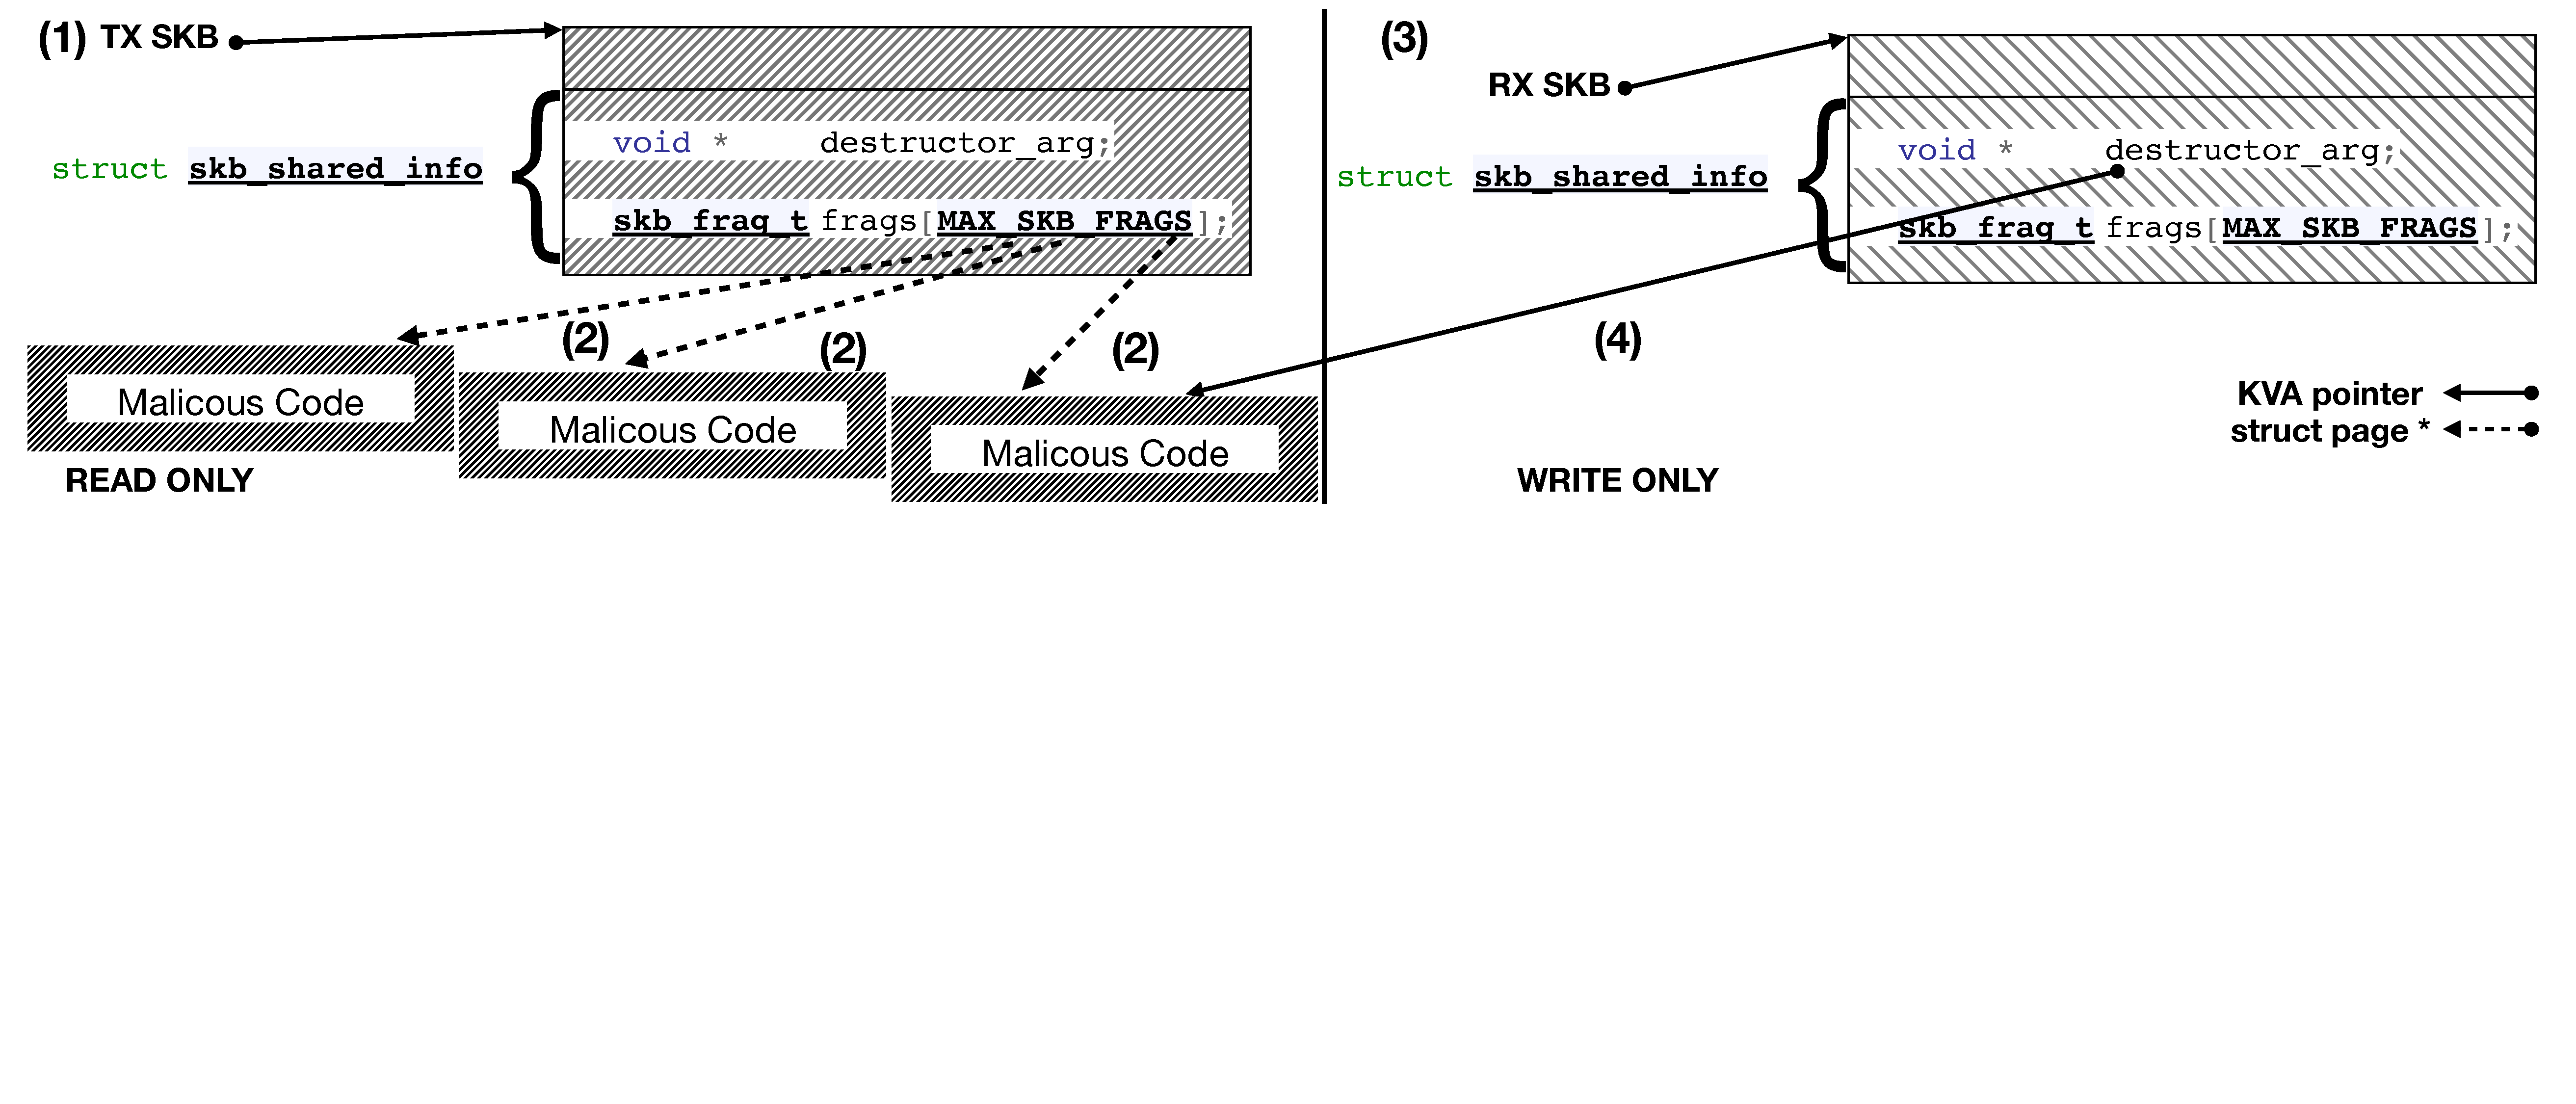
\includegraphics[width=\linewidth]{figs/accomplice.pdf}
    \caption{A TX sk\_buff filled with malicious code used as \means{} for a DMA attack.}
    \label{fig:payload}
\end{figure*}
\subsection{Poisoned TX}\label{sec:posion}

RingFlood (Sec. \ref{sec:ringflod}) allows a NIC to execute arbitrary code with high chances of success. However, the prerequisite is enough information regarding the physical layout of the server and a sufficiently high driver memory footprint. When deducing a valid PFN is not an option (e.g., due to a low memory footprint) another way of acquiring a valid \kva{} is needed.

Since a NIC has READ access to the \shinfo{} of a TX packet, this, in particular, provides the NIC with READ access to the \texttt{frags} (Fig. \ref{fig:payload}) array of \shinfo{}. This array contains \page{} pointers, and thus both leaks kernel pointers that allow the attacker to compromise KASLR, and provides the PFNs of specific pages containing data sent from userspace; pages, the device has READ access to.

%\st{Assuming an unprivileged accomplice (witing or unwitting) can open a UDP/TCP socket in user space, this user can transmit a poisoned ROP buffer. For a ROP attack (where the kernel text offset is required), the NIC spoofs an RX packet with the poisoned ROP stack to the accomplice, which in turn is sent back as a TX packet. Once an accomplice sends the packet,}

Assuming the device can trick a userspace process into echoing a malicious buffer's contents, the device can execute a code injection attack in 4 steps (Fig. \ref{fig:payload}):

\begin{enumerate}
    \item The TX \data{} and the fragments are mapped for the NIC to read.
    \item The NIC spoofs an RX packet and delays the completion notification of the TX packets (so that the \mabaf{} will not be released prematurely).
    \item The NIC identifies the poisoned buffer and translates \page{} to \kva{} (Fig. \ref{fig:mem_model}).
    \item The NIC overwrites \shinfo{} with the \kva{} retrieved during step 2. 
\end{enumerate}

Tricking a userspace process into echoing a malicious buffer's contents can be archived in various ways. For example, a proxy server, a key/value store, streaming service, etc; another type of accomplice can be a cloud VM (e.g., on GCP, AWS, or Azure). A publicly accessible VM may be used to compromise the \emph{host} in the presence of a malicious device.\footnote{Indeed, Googles OpenTitan \cite{opentitan} exemplifies that cloud providers actively worry about root of trust for their servers.}

\textbf{Timing concerns.} A TX completion event that fails to appear in due time will trigger a TX T/O error that flushes all buffers and resets the driver. The T/O is set by the driver usually to a few seconds, which is more than enough to complete the attack.
 
In this scenario, the attacker does not require prior knowledge regarding the physical setup since both \means{} and \motivation{} are provided by the echoing buffer (recall that \oportunity{} is already given, Sec. \ref{sec:shinfo}).  

Namely, the only requirement for the success of this attack is an accomplice, witting (e.g., an unprivileged user) or unwitting (e.g., a proxy server) that can open a socket in user-space. For that matter, a socket in user-space of a \emph{guest machine} makes any cloud VM a valid intrusion tool in the presence of a malicious device.

\smallskip
\noindent\textbf{User buffer.} An attacker could try storing the \mabaf{} and code in user-space. Such and attempt would fail due to SMEP/SMAP \cite{smep} as the kernel will not be able to directly execute user-space code.





